\documentclass[12pt, a4paper]{article}
\usepackage[francais]{babel}
\usepackage{caption}
\usepackage{graphicx}
\usepackage[T1]{fontenc}
\usepackage{listings}
\usepackage{geometry}
\usepackage{minted}
\usepackage{array,multirow,makecell}
\usepackage[colorlinks=true,linkcolor=black,anchorcolor=black,citecolor=black,filecolor=black,menucolor=black,runcolor=black,urlcolor=black]{hyperref}
\setcellgapes{1pt}
\makegapedcells
\usepackage{fancyhdr}
\pagestyle{fancy}
\lhead{}
\rhead{}
\chead{}
\rfoot{\thepage}
\lfoot{Martin Baumgaertner - Mikhaïl Karapetyan}
\cfoot{}
\renewcommand{\footrulewidth}{0.4pt}
\renewcommand{\headrulewidth}{0.4pt}
\renewcommand{\listingscaption}{Code}
\renewcommand{\listoflistingscaption}{Table des codes}
% \usepackage{mathpazo} --> Police à utiliser lors de rapports plus sérieux

\begin{document}
\begin{titlepage}
	\newcommand{\HRule}{\rule{\linewidth}{0.5mm}} 
	\center 
	\textsc{\LARGE iut de colmar}\\[6.5cm] 
	\textsc{\Large TP 1 - configuration d'un point d'accès wifi}\\[0.5cm] 
	\textsc{\large Année 2022-23}\\[0.5cm]
	\HRule\\[0.75cm]
	{\huge\bfseries R301 - Réseaux de campus}\\[0.4cm]
	\HRule\\[1.5cm]
	\textsc{\large martin baumgaertner - mikhaïl karapetyan}\\[6.5cm] 

	\vfill\vfill\vfill
	{\large\today} 
	\vfill
\end{titlepage}
\newpage
\tableofcontents
\listoffigures
\listoflistings
\newpage
\section{Création d'un nouvel utilisateur et désactivation de l'utilisateur par défaut}
    \subsection{Donnez la signification de \textit{"aaa"}}
    AAA est un protocole de sécurisation des équipements dont les trois lettres signifient : Authentication, Authorization et Accounting.\\
    \begin{itemize}
        \item L’Authentication (authentification en français) fait référence à la capacité que l’équipement aura de vérifier l’identité de l’utilisateur. C’est un processus qui va décider si un utilisateur donné peut accéder au réseau ou à l’équipement sur lequel AAA est configuré.\\
        \item L’Authorization (autorisation en français) fait quant à lui référence aux ressources auxquelles l’utilisateur va pouvoir accéder, et les opérations qu’il va être en mesure d’effectuer.\\
        \item L’Accounting (gestion des comptes) concerne les données et les informations se rapportant au profil de l’utilisateur.\\
    \end{itemize}

    \subsection{Expliquez précisement la signification de chaque ligne}
    \begin{itemize}
        \item \texttt{aaa-new model} : permet de créer un nouveau modèle AAA.
        \item \texttt{aaa authorization exec default local} : permet de définir le modèle d'autorisation pour les commandes exécutées en mode exec.
        \item \texttt{username toto privilege 15 password tototo} : permet de créer un nouvel utilisateur avec le nom \textit{toto} et le mot de passe \textit{tototo}.
        \item \texttt{no username Cisco} : permet de désactiver l'utilisateur par défaut.
        \item \texttt{no enable secret} : permet de désactiver le mot de passe par défaut.
    \end{itemize}

\section{Activation du SSH et connexion à la borne}
    \subsection{Exportez la configuration obtenue dans votre CR}
    \begin{listing}[H]
        \caption{Partie 1 de la configuration }
        \label{lst:conf}
        \begin{minted}{bash}
    RT222-BK#show running-config
    Building configuration...

    Current configuration : 1341 bytes
    !
    version 12.3
    no service pad
    service timestamps debug datetime msec
    service timestamps log datetime msec
    service password-encryption
    !
    hostname RT222-BK
    !
    !
    ip subnet-zero
    !
    !
    aaa new-model
    !
    !
    aaa authorization exec default local
    aaa session-id common
    !
    !
    username toto privilege 15 password 7 0835435A060D0A031D
    username admin privilege 15 password 7 14031D1F0310253F2B
    !
    bridge irb
    !
    !
        \end{minted}
    \end{listing}

    \begin{listing}[H]
        \caption{Partie 2 de la configuration }
        \label{lst:conf2}
        \begin{minted}{bash}
    interface Dot11Radio0
    no ip address
    no ip route-cache
    shutdown
    speed basic-1.0 basic-2.0 basic-5.5 6.0 9.0 basic-11.0 12.0 
    18.0 24.0 36.0 48.0 54.0
    station-role root
    bridge-group 1
    bridge-group 1 subscriber-loop-control
    bridge-group 1 block-unknown-source
    no bridge-group 1 source-learning
    no bridge-group 1 unicast-flooding
    bridge-group 1 spanning-disabled
    !
    interface FastEthernet0
    no ip address
    no ip route-cache
    duplex auto
    speed auto
    bridge-group 1
    no bridge-group 1 source-learning
    bridge-group 1 spanning-disabled
    hold-queue 160 in
    !
    interface BVI1
    ip address dhcp
    ip access-group 25 in
    no ip route-cache
    !
    ip http server
    no ip http secure-server
    ip http help-path http://www.cisco.com/warp/public/779/smbiz/prodconfig/
    help/eag
    !
        \end{minted}
    \end{listing}

    \begin{listing}[H]
        \caption{Partie 3 de la configuration }
        \label{lst:conf3}
        \begin{minted}{bash}
    access-list 25 permit 10.129.10.207
    access-list 25 deny   any
    !
    control-plane
    !
    bridge 1 route ip
    !
    !
    !         
    line con 0
    line vty 0 4
    transport input ssh
    line vty 5 15
    transport input ssh
    !
    end
        \end{minted}
    \end{listing}

\section{Configuration WiFi de base via l'interface web et la console}
    \subsection{Mode Open}
        \subsubsection{Faites une capture d'écran}
        \begin{figure}[H]
            \centering
            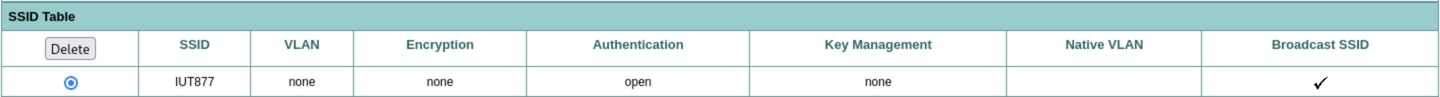
\includegraphics[width=1\textwidth]{img/config-express.png}
            \caption{Configuration EXPRESS}
            \label{fig:exp}
        \end{figure}
        Pour que cela fonctionne, nous avons dû mettre en route notre interface.
        \begin{figure}[H]
            \centering
            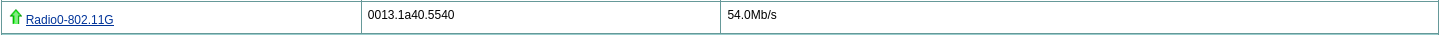
\includegraphics[width=1\textwidth]{img/int.png}
            \caption{Interface}
            \label{fig:int}
        \end{figure}

        \subsubsection{Avec \texttt{sh running-config} faites une capture d'écran}
        \begin{figure}[H]
            \centering
            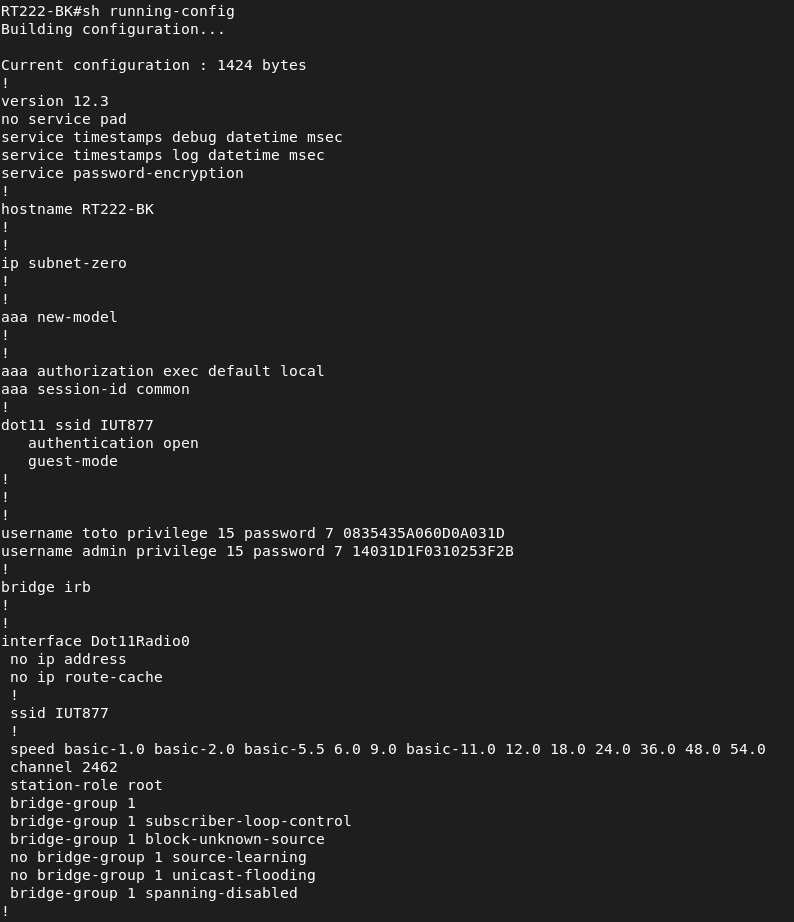
\includegraphics[width=0.8\textwidth]{img/part1.png}
            \caption{Configuration partie 1}
            \label{fig:sh1}
        \end{figure}
        \begin{figure}[H]
            \centering
            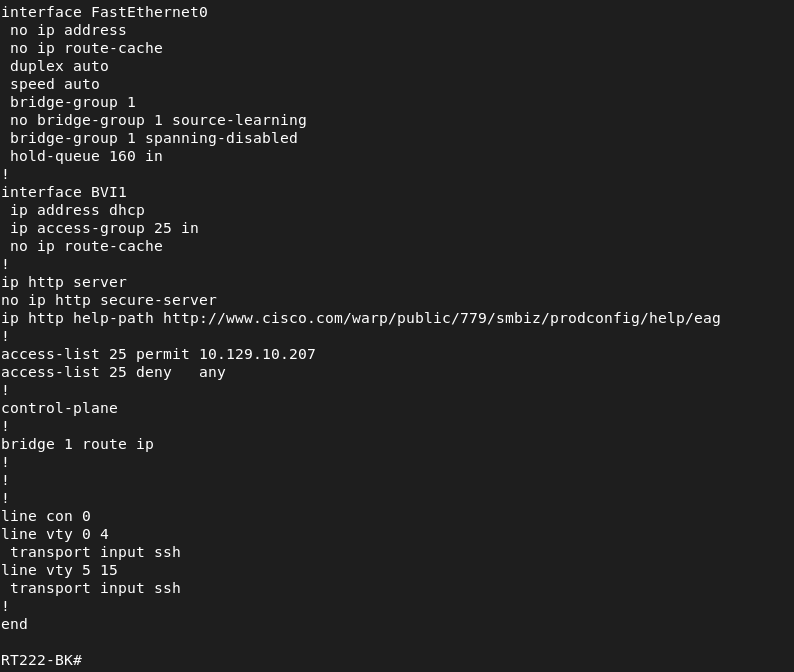
\includegraphics[width=1\textwidth]{img/part2.png}
            \caption{Configuration partie 2}
            \label{fig:sh2}
        \end{figure}

        \subsubsection{Indiquez le rôle exact des options \texttt{guest-mode, authentication open} et \texttt{no shutdown}}
        \begin{itemize}
            \item \texttt{guest-mode} : permet de créer un réseau invité.
            \item \texttt{authentication open} : permet de désactiver l'authentification.
            \item \texttt{no shutdown} : permet de mettre en route l'interface.
        \end{itemize}


    \subsection{Mode WEP}

        \subsubsection{Faites une capture d'écran}
        \begin{figure}[H]
            \centering
            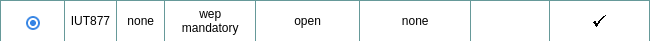
\includegraphics[width=1\textwidth]{img/mode-wep.png}
            \caption{Configuration WEP}
            \label{fig:wep}
        \end{figure}

        \subsubsection{Avec \texttt{sh running-config} faites une capture d'écran}
        \begin{figure}[H]
            \centering
            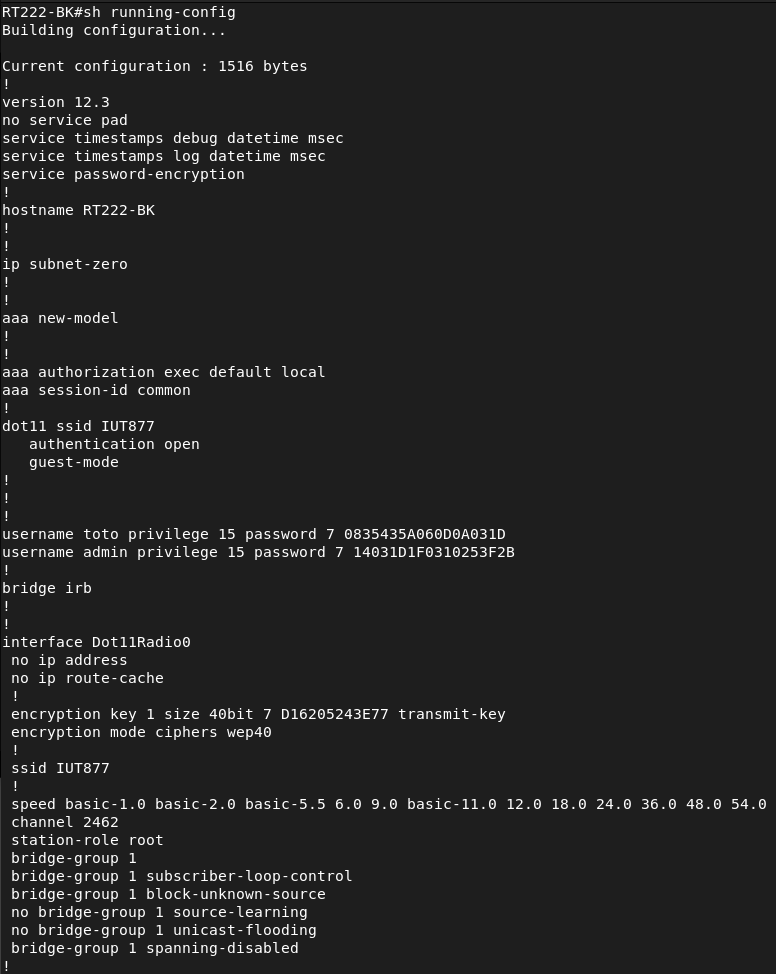
\includegraphics[width=0.7\textwidth]{img/config-part1.png}
            \caption{Configuration partie 1}
            \label{fig:conf1}
        \end{figure}
        \begin{figure}[H]
            \centering
            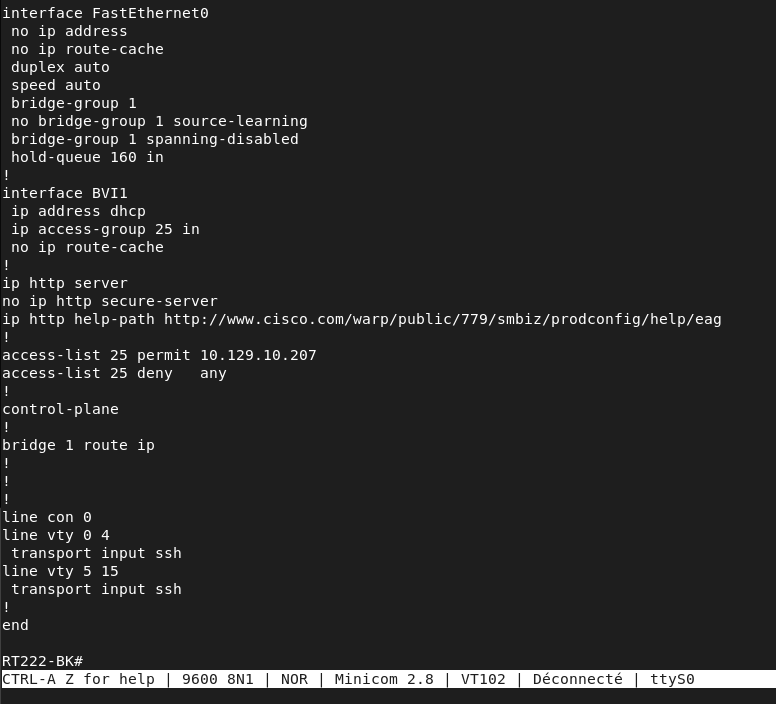
\includegraphics[width=1\textwidth]{img/config-part2.png}
            \caption{Configuration partie 2}
            \label{fig:conf2}
        \end{figure}


    \subsection{Mode WPA - PSK}

        \subsubsection{Faites une capture d'écran}
        \begin{figure}[H]
            \centering
            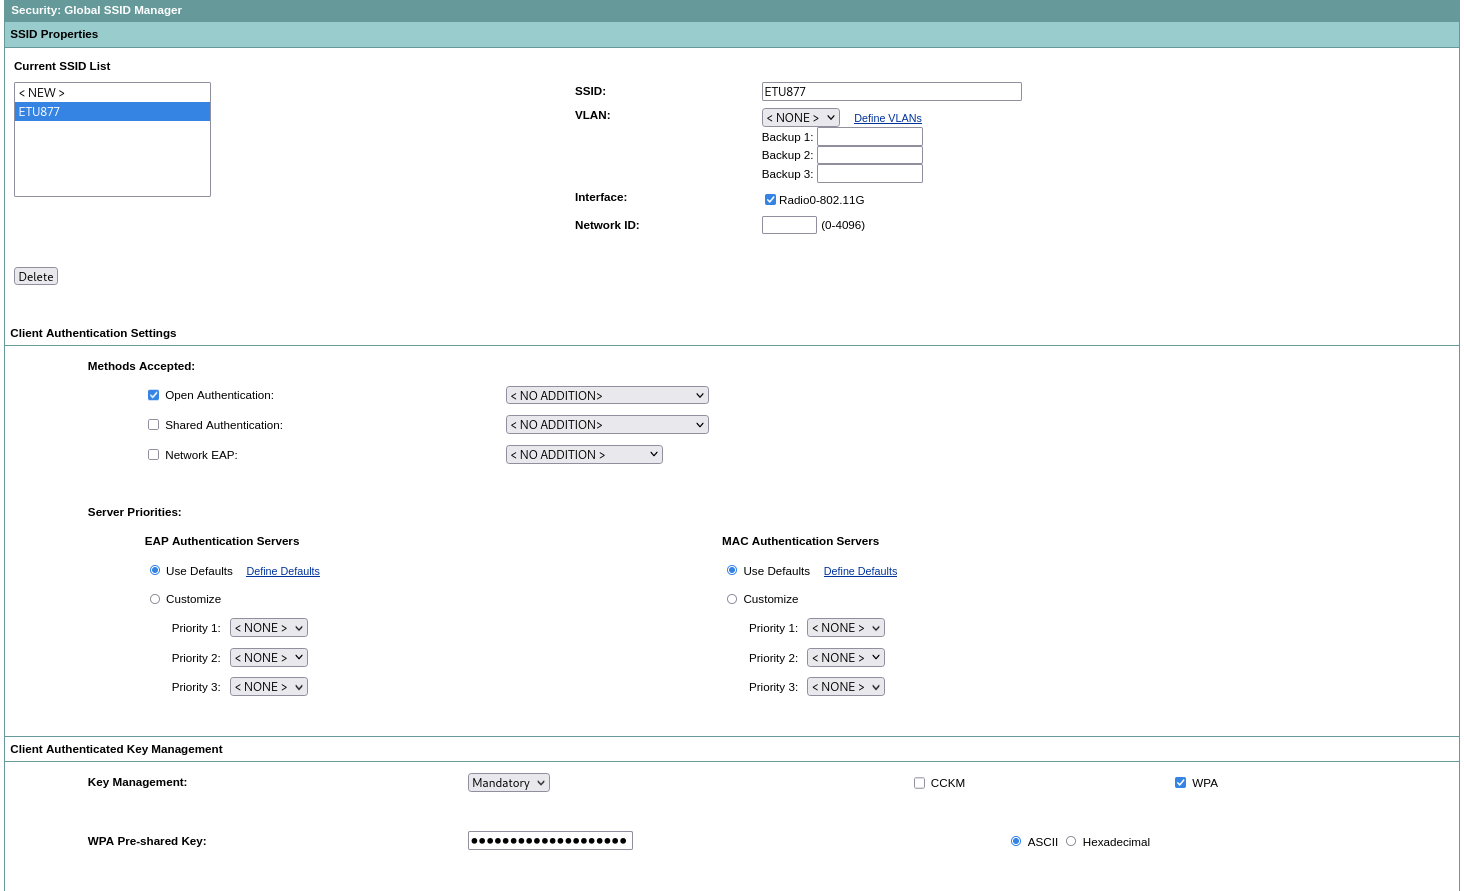
\includegraphics[width=0.8\textwidth]{img/ssid-manage1.png}
            \caption{Configuration SSID Manager partie 1}
            \label{fig:ssid1}
        \end{figure}
        \begin{figure}[H]
            \centering
            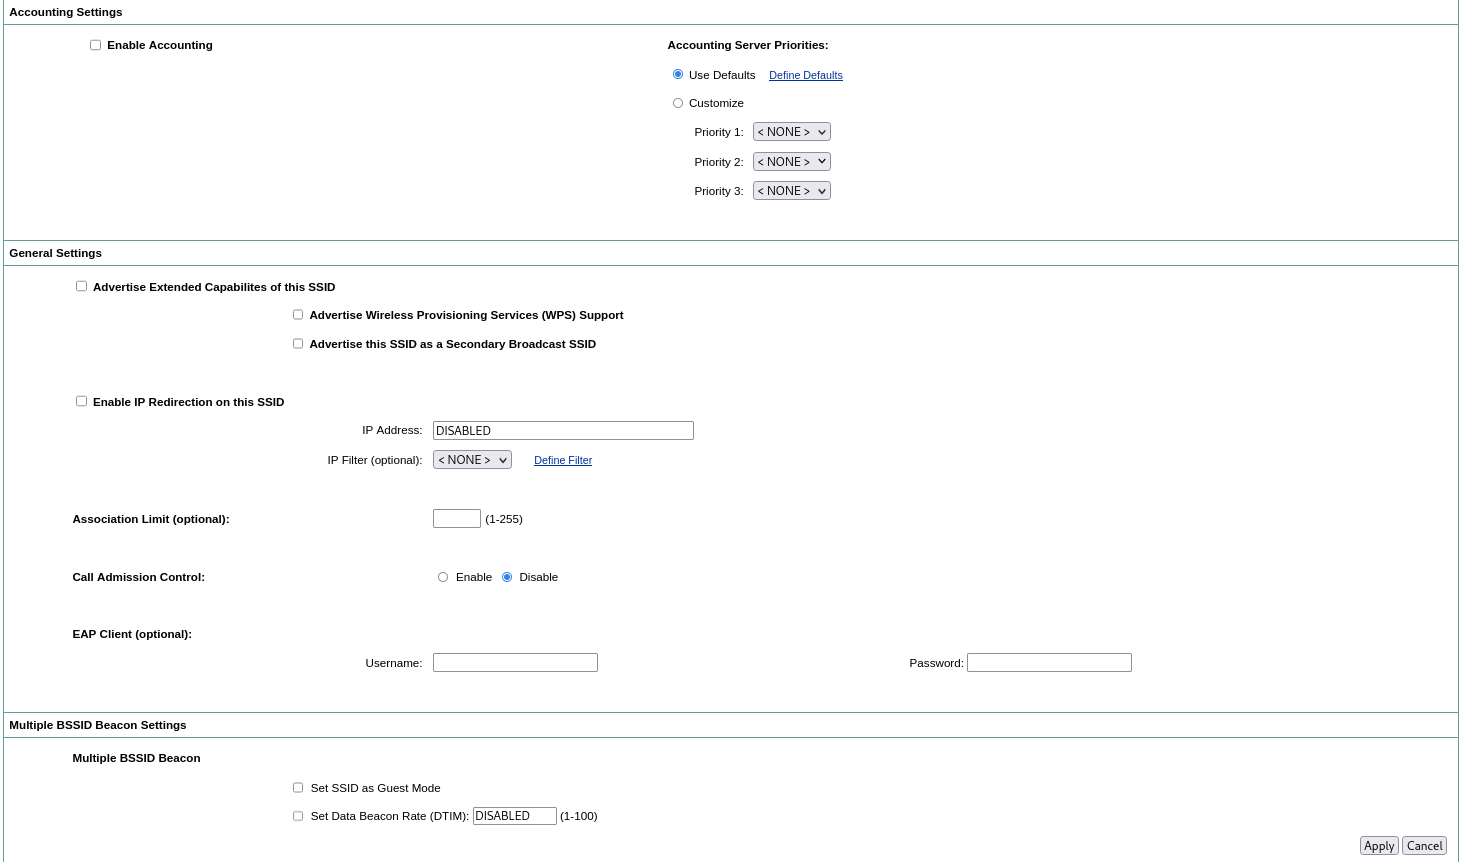
\includegraphics[width=0.8\textwidth]{img/ssid-manage2.png}
            \caption{Configuration SSID Manager partie 2}
            \label{fig:ssid2}
        \end{figure}

        \subsubsection{Faites une capture d'écran}
        \begin{figure}[H]
            \centering
            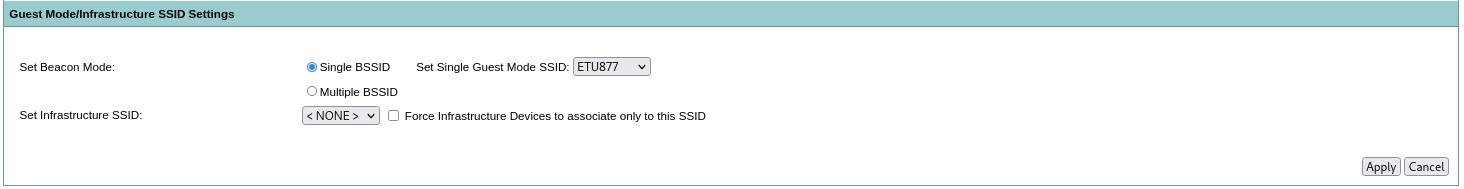
\includegraphics[width=1\textwidth]{img/config-manage3.png}
            \caption{Configuration SSID Manager après modification}
            \label{fig:ssid3}
        \end{figure}

        \subsubsection{Avec \texttt{sh running-config} faites une capture d'écran}
        \begin{figure}[H]
            \centering
            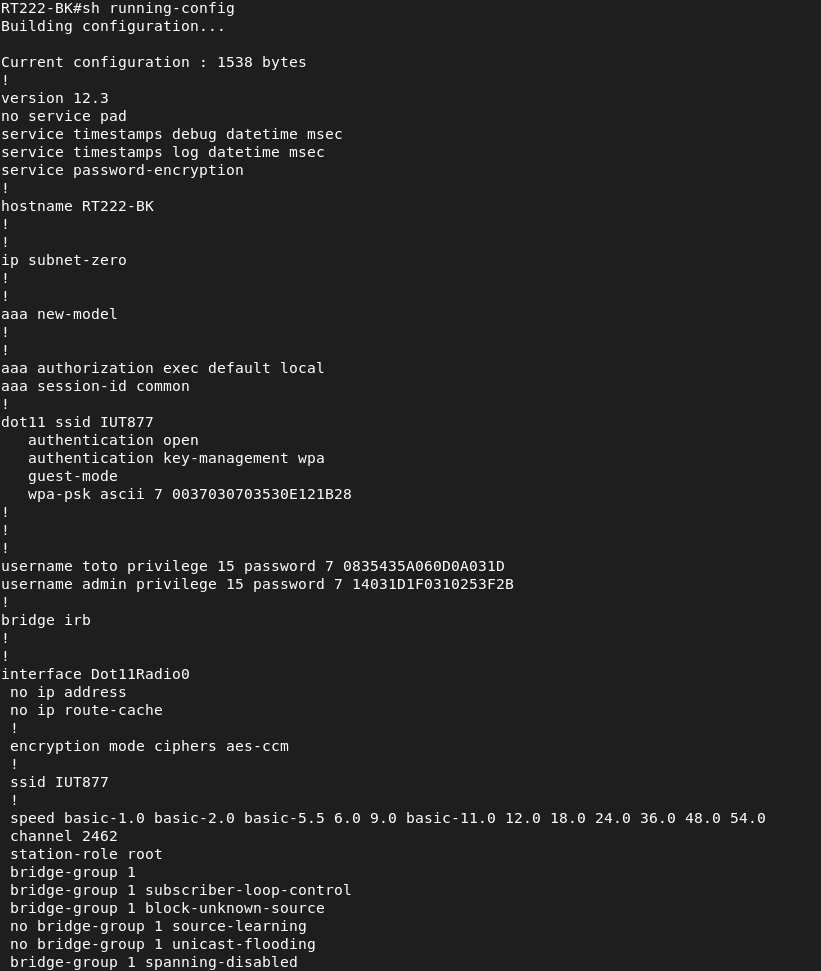
\includegraphics[width=0.7\textwidth]{img/configg-part1.png}
            \caption{Configuration \texttt{sh running-config} partie 1}
            \label{fig:configg1}
        \end{figure}
        \begin{figure}[H]
            \centering
            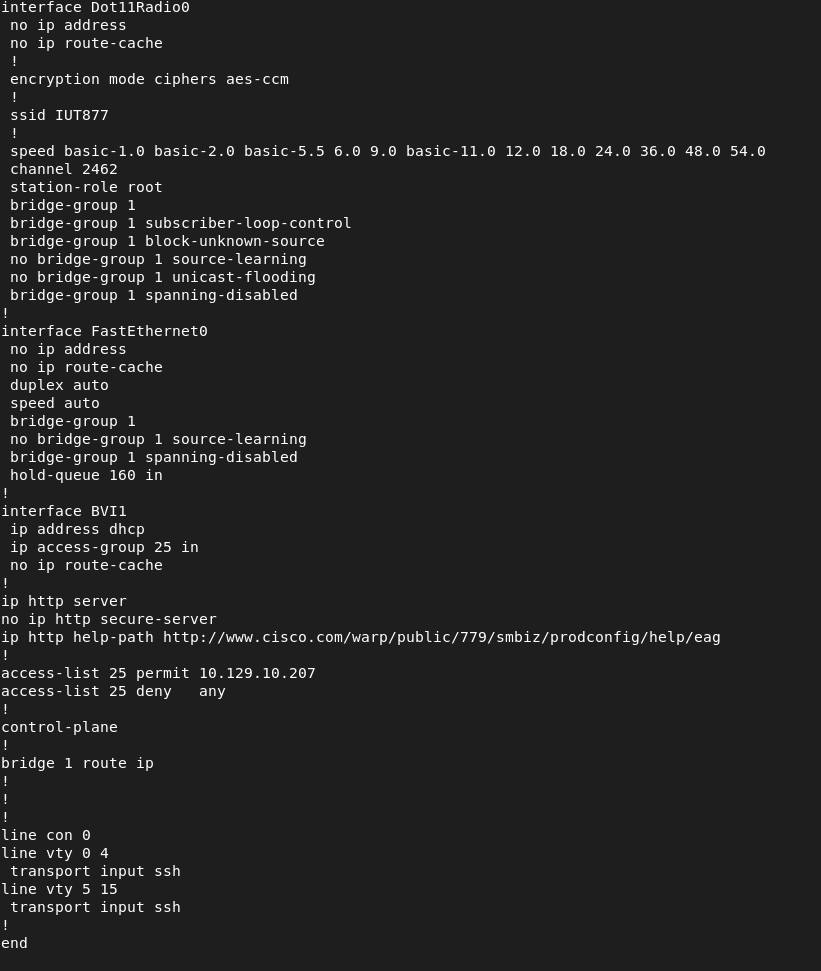
\includegraphics[width=1\textwidth]{img/configg-part2.png}
            \caption{Configuration \texttt{sh running-config} partie 2}
            \label{fig:configg2}
        \end{figure}

    \subsection{Filtrage des adresses MAC}
        \subsubsection{Via interface WEB}
        \begin{figure}[H]
            \centering
            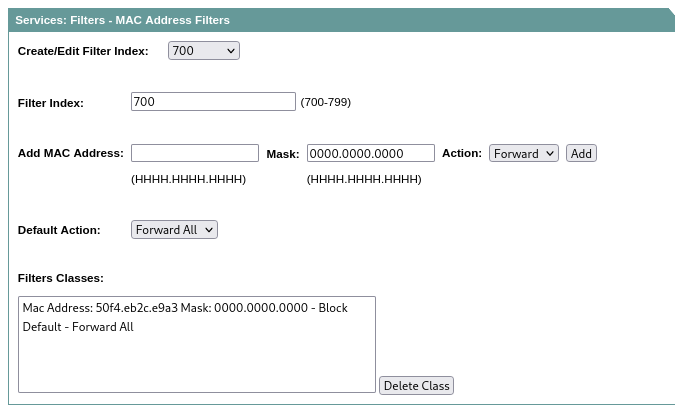
\includegraphics[width=0.6\textwidth]{img/filtrage-mac.png}
            \caption{Configuration du filtrage MAC}
            \label{fig:mac}
        \end{figure}
        \begin{figure}[H]
            \centering
            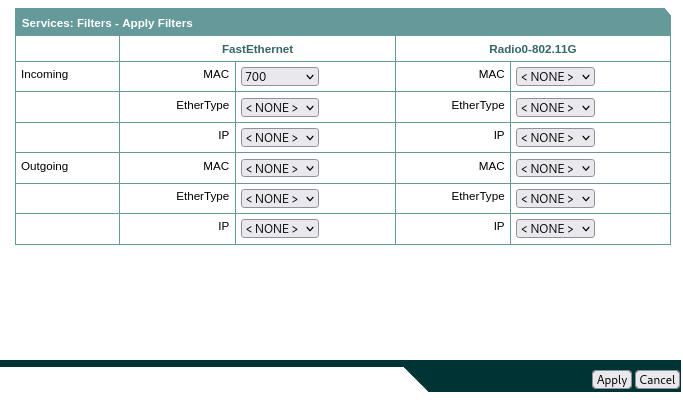
\includegraphics[width=0.6\textwidth]{img/filtrage-mac2.png}
            \caption{Configuration du filtrage MAC}
            \label{fig:mac2}
        \end{figure}

        \subsubsection{En console}
        \begin{figure}[H]
            \centering
            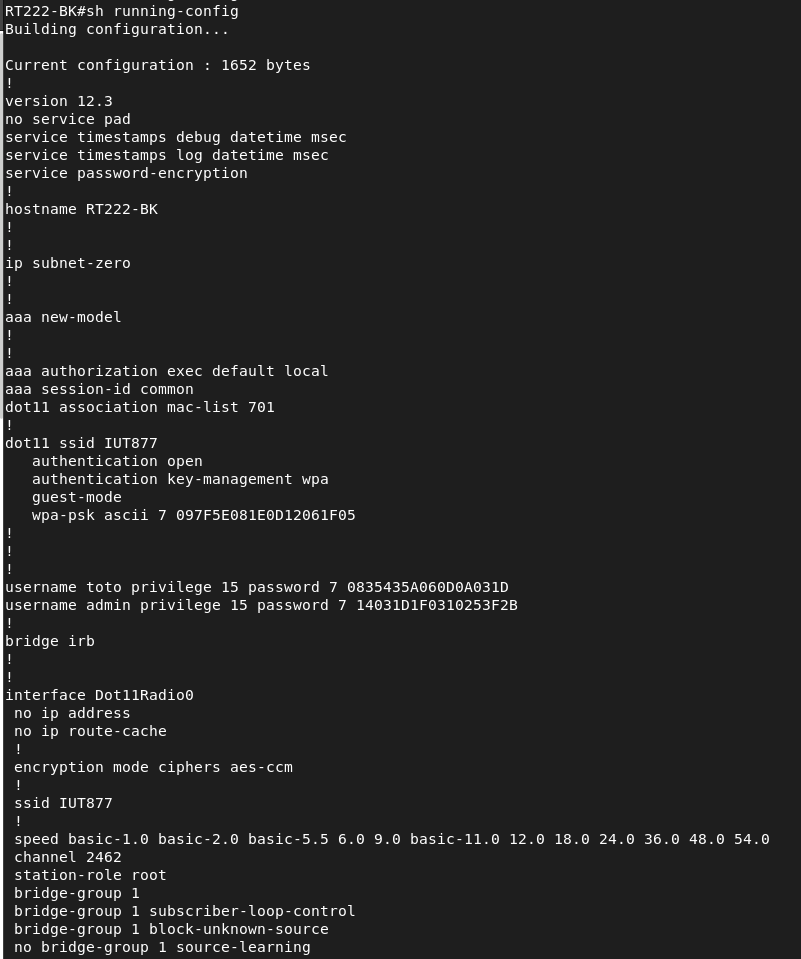
\includegraphics[width=0.5\textwidth]{img/console1.png}
            \caption{Configuration du filtrage MAC en mode console partie 1}
            \label{fig:console1}
        \end{figure}
        \begin{figure}[H]
            \centering
            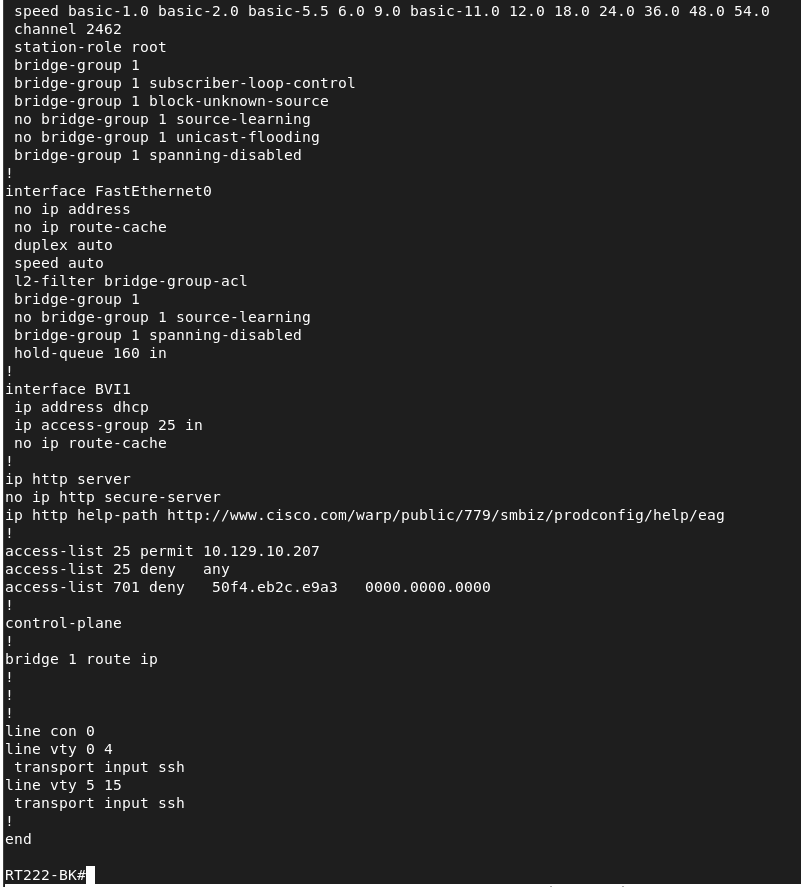
\includegraphics[width=0.4\textwidth]{img/console2.png}
            \caption{Configuration du filtrage MAC en mode console partie 2}
            \label{fig:console2}
        \end{figure}


    
\end{document}